\documentclass[11pt,a4paper]{article}

% ---------- arxiv-style preamble (xelatex; emoji-native) ----------
\usepackage[margin=1in]{geometry}
\usepackage{amsmath,amssymb,amsthm}
\usepackage{graphicx}
\usepackage{booktabs}
\usepackage{siunitx}
\usepackage{hyperref}
\usepackage{xcolor}
\usepackage[numbers,sort&compress]{natbib}
\usepackage{tikz}
\usetikzlibrary{positioning,arrows.meta,fit,backgrounds}
\usepackage{pgfplots}
\pgfplotsset{compat=1.18}
\usepgfplotslibrary{fillbetween}
\usepackage{caption}
\captionsetup{font=small,labelfont=bf}
\usepackage{array}

\hypersetup{
  colorlinks=true,
  linkcolor=blue!50!black,
  citecolor=blue!50!black,
  urlcolor=blue!50!black
}

% ---------- tier badges (engine-agnostic colored discs) ----------
\newcommand{\tierdisc}[1]{\textcolor{#1}{\rule[0.05ex]{1.0ex}{1.0ex}}}
\newcommand{\tierBlue}{\tierdisc{blue!70!black}}
\newcommand{\tierGreen}{\tierdisc{green!60!black}}
\newcommand{\tierYellow}{\tierdisc{yellow!85!black}}
\newcommand{\tierOrange}{\tierdisc{orange!90!black}}
\newcommand{\tierRed}{\tierdisc{red!80!black}}

\newcommand{\fs}{f_{\mathrm{s}}}
\newcommand{\fq}{f_{\mathrm{q}}}
\newcommand{\Stot}{S_{\mathrm{total}}}
\newcommand{\fclear}{f_{\mathrm{clear}}}
\newcommand{\pdep}{p_{\mathrm{dep}}}

\title{
  \textbf{🧬 Senolytic Selectivity Is a Differential-Dependency Quantity,
  Not a Binding Affinity} \\[6pt]
  \large A Closed-Form Selectivity Law, a Heterogeneity Ceiling Theorem,
  and an Orthogonal Three-Axis AND-Gate Design (SENOLYX-AG)
  for Regenerative-Niche Senescent Fibroblasts
}

\author{
  \texttt{demiurge} maintainers\\
  \normalsize\textit{dancinlab}\\[2pt]
  \normalsize\href{https://github.com/dancinlab/demiurge}{\texttt{github.com/dancinlab/demiurge}}
}

\date{\today}

\begin{document}
\maketitle

\begin{figure}[h]
\centering

\includegraphics[width=0.82\textwidth]{figures/cover.png}
\caption{The SENOLYX-AG concept (fal.ai/FLUX-generated cover). A healthy cell
(left) engages at most one recognition lock and is spared; a senescent cell
(right) engages all three orthogonal locks (two surface, one lysosomal) and is
cleared. Selectivity is the multiplicative AND of independent recognition axes.}
\label{fig:cover}
\end{figure}

% =========================================================================
\begin{abstract}
We report a closed-form theory of \emph{senolytic selectivity} --- the
therapeutic window separating senescent-cell killing from healthy-cell
toxicity --- together with a concrete, in-silico-supported molecular design
that follows from it. The work was prompted by a campaign wall: an absolute
binding free-energy (ABFE) effort to optimize senolytic candidates plateaued
at the force-field ceiling. We show this was not a numerical failure but a
\emph{category error}. Two independent ``wrong axes'' are identified and ruled
out. First, selectivity is governed by the \emph{differential anti-apoptotic
dependency} between senescent and quiescent cells, $\fs/\fq$, and the absolute
binding free energy $\Delta G_{\mathrm{bind}}$ \emph{cancels} from the
selectivity condition --- explaining mechanistically why the ABFE axis was
uninformative, and corroborated by the textbook navitoclax counterexample
(tightest BCL-x$_{\mathrm L}$ affinity, narrowest clinical window). Second, the
downstream ``\% senescent cells cleared $\to$ regeneration'' transfer function
is non-monotone and not literature-grounded; clearance-\% is itself a poor gate
variable, replaced here by a functional $\eta_{\mathrm{neo}}$ pharmacodynamic
model anchored to two real clinical outcomes (UBX1325 success, UBX0101
failure). We derive a selectivity law $x^{*}=(B-A)/(f\,B)$ with a
selectivity condition $\Delta x^{*}>0$; a heterogeneity \emph{ceiling theorem}
$\fclear(T)\le\pdep(T)<1$ for any single-target agent (no universal
senescence dependency exists); and a multiplicative \emph{escape}
$\Stot=\prod_i S_i$ available only on orthogonal recognition axes. A direct
numerical evaluation (the \texttt{S1} index) shows a single marker is net
anti-selective ($0.92\times$), a two-axis gate collapses below $2\times$ under
modest axis correlation, and only a \emph{three-axis} AND-gate
(uPAR\,$\times$\,DPP4\,$\times$\,SA-$\beta$-gal) is robust ($23\times$ median,
adverse-box minimum $4.34\times$). Combined with a kill-axis term
$\fs/\fq\approx1.6\times$, the realistic total selectivity is
$\sim$\,$13.5$--$26\times$. The resulting design, \textbf{SENOLYX-AG}, is a
galacto-caged BCL-x$_{\mathrm L}$/MCL-1 PROTAC inside a surface-marker-gated
local-delivery particle, first-targeted to the periodontal niche. Every
molecular component is published chemistry; the novelty is the composition.
The single remaining make-or-break unknown is the cross-axis correlation
$\rho$, which we bound by regulatory-hub independence and which a single
three-color flow-cytometry experiment would close. All claims are in-silico /
literature-grounded; wet-lab confirmation is explicitly downstream.
\end{abstract}

\tableofcontents
\bigskip

% =========================================================================
\section{Introduction}
\label{sec:intro}

Senolytics --- drugs that selectively eliminate senescent cells --- are a
leading geroscience strategy: clearing senescent cells rejuvenates tissue and
extends healthspan in mice \citep{baker2011,baker2016}. Yet after a decade no
senolytic has cleared a pivotal clinical trial. The two highest-profile
controlled readouts to date are \emph{negative or mixed}: UBX0101 (an
MDM2--p53 senolytic) failed its Phase~2 osteoarthritis endpoint, while UBX1325
(a BCL-x$_{\mathrm L}$ senolytic) succeeded in the retina only via local
intravitreal delivery \citep{ubx1325}. The field's central unsolved problem is
not \emph{potency} but \emph{selectivity}: the therapeutic window between
killing senescent cells and harming healthy ones.

This paper began as a debugging exercise. A computational campaign
(\texttt{SENOLYX}) attempted to rank senolytic candidates by absolute binding
free energy (ABFE) using openmmtools double-decoupling. The effort plateaued:
the force field imposed a precision ceiling, and the rankings did not track
known selectivity. Rather than treat this as a convergence problem, we asked
whether \emph{affinity is the wrong axis entirely}. It is. We then asked
whether the downstream cure metric (\% cells cleared) was the right gate. It is
not. Removing both wrong axes leaves a clean, closed-form theory of selectivity
and a concrete design that the theory recommends.

\paragraph{Contributions.}
\begin{enumerate}
\item A closed-form \textbf{selectivity law} showing selectivity is a
  differential-dependency quantity, with the binding affinity provably absent
  (\S\ref{sec:law}).
\item A \textbf{heterogeneity ceiling theorem}: no single-target senolytic can
  selectively clear all senescent cells, because no survival dependency is
  universal (\S\ref{sec:ceiling}).
\item A \textbf{multiplicative escape}: only an orthogonal AND-gate multiplies
  selectivity; a direct numerical evaluation shows three axes are required for
  robustness (\S\ref{sec:escape},\,\S\ref{sec:s1}).
\item A correction of the downstream \textbf{gate variable} from clearance-\%
  to a functional $\eta_{\mathrm{neo}}$ model anchored to clinical outcomes
  (\S\ref{sec:pd}).
\item \textbf{SENOLYX-AG}: a concrete, buildable, in-silico-supported design
  with a single named make-or-break experiment (\S\ref{sec:design}).
\end{enumerate}

% =========================================================================
\section{Hypothesis and pre-registered falsifiers}
\label{sec:hypothesis}

We pre-register the following falsifiable hypotheses before presenting
measurements.

\begin{description}
\item[H1 (affinity-orthogonality).] Senolytic selectivity is determined by the
  differential anti-apoptotic dependency $\fs/\fq$, not by absolute binding
  affinity. \textbf{Falsifier:} if a high-affinity BH3 mimetic with no
  dependency differential ($\fs=\fq$) achieves senescent selectivity, or if
  absolute affinity rank-orders the known senolytic windows better than the
  dependency differential, H1 is false.
\item[H2 (heterogeneity ceiling).] For any single targeted survival pathway
  $T$, the selectively clearable senescent fraction obeys
  $\fclear(T)\le\pdep(T)<1$. \textbf{Falsifier:} a single survival dependency
  present in essentially every senescent cell type (a ``universal senolytic
  target'') would refute the ceiling.
\item[H3 (multiplicative escape).] Selectivity multiplies across statistically
  independent recognition axes, $\Stot=\prod_i S_i$. \textbf{Falsifier:} if the
  candidate recognition axes are strongly co-regulated (correlation
  $\rho\to1$), the product collapses to a single axis and the AND-gate provides
  no advantage.
\item[H4 (gate-variable).] Tissue regeneration ($\eta_{\mathrm{neo}}$) is
  governed by which causal SASP-driving subtype is cleared, local exposure, and
  re-accumulation --- not by the global clearance fraction. \textbf{Falsifier:}
  a monotone clearance-\% $\to$ regeneration relationship with a reproducible
  threshold would restore clearance-\% as the gate.
\end{description}

% =========================================================================
\section{Methods}
\label{sec:methods}

\paragraph{Multi-lens evidence synthesis.}
Each hypothesis was probed by an independent literature-and-modeling lens
(a background research agent), constrained to (i) read the primary literature
as an answer key before modeling, (ii) report a falsifiable verdict tier, and
(iii) state honestly what is measured versus inferred. Verdict tiers follow the
project rubric: \tierBlue{}~formal/closed-form, \tierGreen{}~model-verified,
\tierYellow{}~citation-only, \tierOrange{}~inconclusive, \tierRed{}~closed-negative.

\paragraph{Numerical models (mini-free, \texttt{numpy}/\texttt{scipy}).}
The selectivity index \texttt{S1} (\S\ref{sec:s1}) and the apoptotic-commitment
threshold model (\S\ref{sec:law}) are deterministic and reproduced
independently. The $\eta_{\mathrm{neo}}$ pharmacodynamic model
(\S\ref{sec:pd}) is anchor-calibrated and checked for monotonicity in all
inputs. We deliberately \emph{demote} ABFE/MD from a ranking tool to a binary
``does the caged warhead still bind'' confirmation, since the selectivity
quantities are ratios in which force-field systematic error largely cancels.

\paragraph{Honesty boundary (in-silico vs wet-lab).}
Throughout, in-silico evidence decides directionality, robustness, and order of
magnitude of every selectivity factor, the AND-gate logic, and the causal
structure of the cure model. It does \emph{not} deliver calibrated absolute
potencies or efficacy; those are wet-lab, treated as downstream confirmation.

% =========================================================================
\section{The selectivity law (H1)}
\label{sec:law}

Model a cell's commitment to mitochondrial outer-membrane permeabilization
(MOMP, i.e.\ apoptotic death) as a threshold competition between an activator
BH3 stress $A$ and an anti-apoptotic buffer $B$, of which a fraction $f$ is
carried by the drug-targeted protein. Under drug occupancy $x$ the available
buffer is $B(1-fx)$, and the cell dies when

\begin{equation}
A - B\,(1 - f\,x) > \theta ,
\label{eq:momp}
\end{equation}

with $\theta$ the permeabilization threshold. The occupancy required to kill
(taking $\theta=0$) is

\begin{equation}
\boxed{\;x^{*} = \dfrac{B - A}{f\,B}\;}
\label{eq:xstar}
\end{equation}

A senolytic is \emph{selective} when senescent cells cross the kill threshold
at a lower occupancy (hence dose) than quiescent cells, i.e.\ when

\begin{equation}
\Delta x^{*} \;=\; \underbrace{\frac{B_{\mathrm q}-A_{\mathrm q}}{\fq\,B_{\mathrm q}}}_{\text{quiescent}}
\;-\;
\underbrace{\frac{B_{\mathrm s}-A_{\mathrm s}}{\fs\,B_{\mathrm s}}}_{\text{senescent}}
\;>\;0 .
\label{eq:deltax}
\end{equation}

The dominant lever is $\fs\gg\fq$: senescent cells funnel survival through a
single druggable buffer. \textbf{Crucially, the binding affinity
$\Delta G_{\mathrm{bind}}$ does not appear in Eq.~\eqref{eq:deltax}.} Affinity
only maps a given occupancy $x$ to a dose; it cannot create a window. This is
the mechanistic root of the ABFE wall: a quantity absent from the selectivity
condition cannot rank selectivity.

A Monte-Carlo evaluation of Eq.~\eqref{eq:momp} (40{,}000 cells) with both
populations alive at baseline confirms the algebra: with senescent cells
\emph{less} primed overall ($A-B=-0.40$ vs $-0.30$) but BCL-x$_{\mathrm L}$-routed
($\fs=0.75,\fq=0.25$), the therapeutic window peaks at $+0.782$, and
$\Delta x^{*}=+0.756>0$. Removing the differential ($\fq=\fs$) drives the window
\emph{negative} ($-0.03$ to $-0.11$): the drug then preferentially kills healthy
cells. Selectivity is impossible without the dependency differential.

\paragraph{Empirical anchor.}
This is the closed-form of an empirical result: \citet{sotogamez2024} show that
specific BCL-x$_{\mathrm L}$ dependency (HRKy BH3 profiling), not overall
priming, predicts senolytic killing --- senescent cells are in fact \emph{less}
primed overall, yet their dependency \emph{routes onto} BCL-x$_{\mathrm L}$. The
therapeutic-index-as-differential-priming principle traces to
\citet{vo2011,montero2018}.

\paragraph{Corpus test (H1).}
Across the known senolytic corpus, affinity rank inverts selectivity rank. The
decisive case is navitoclax \citep{chang2016}: among the tightest
BCL-x$_{\mathrm L}$ binders, yet the narrowest window (dose-limiting
thrombocytopenia, on-target platelet BCL-x$_{\mathrm L}$). Agents that widen the
window do so by gating, not by higher affinity (Table~\ref{tab:corpus}). H1 is
\emph{supported}; its falsifier (affinity beating the differential) is not
observed.

\begin{table}[t]
\centering
\caption{Senolytic corpus: affinity $\neq$ selectivity. High-affinity
BCL-x$_{\mathrm L}$ binding (navitoclax) gives the narrowest window; window
widening comes from gating/local delivery, not affinity.}
\label{tab:corpus}
\small
\begin{tabular}{@{}llll@{}}
\toprule
Agent & Target / SCAP & Window / DLT & Status \\
\midrule
Navitoclax \citep{chang2016} & BCL-2/x$_{\mathrm L}$/w (sub-nM) & narrow (thrombocytopenia) & on-target tox \\
D+Q \citep{zhu2015} & multi-kinase / BCL-x$_{\mathrm L}$ & broad, partial (30--70\%) & feasibility trials \\
A-1331852 & BCL-x$_{\mathrm L}$-selective & platelet risk & preclinical \\
Fisetin \citep{yousefzadeh2018} & poly-pharmacology & wide, weak & trials \\
UBX0101 \citep{jeon2017} & MDM2--p53 & local (intra-articular) & \tierRed{} Ph2 OA fail \\
UBX1325 \citep{ubx1325} & BCL-x$_{\mathrm L}$ (intravitreal) & local, spared & \tierGreen{} Ph2 win \\
Nav-Gal \citep{navgal2020} & BCL-x$_{\mathrm L}$ + SA-$\beta$-gal gate & widened ($16\!\to\!35\times$) & preclinical \\
uPAR CAR-T \citep{amor2020} & uPAR surface gate & orthogonal & preclinical \\
\bottomrule
\end{tabular}
\end{table}

% =========================================================================
\section{The heterogeneity ceiling theorem (H2)}
\label{sec:ceiling}

For a single targeted survival pathway $T$, the maximum \emph{selectively}
clearable senescent fraction is bounded:

\begin{equation}
\boxed{\;\fclear(T) \;\le\; \pdep(T)\cdot F_b(D_{\mathrm{tox}})\;}
\label{eq:ceiling}
\end{equation}

where $\pdep(T)$ is the fraction of the senescent population whose
survival-critical dependency is $T$, and $F_b(D_{\mathrm{tox}})$ is the
cumulative buffer distribution evaluated at the maximum safe dose
$D_{\mathrm{tox}}=\mathrm{TW}\cdot\mathrm{EC50}_{\mathrm{sen}}$, with the
therapeutic window $\mathrm{TW}=\mathrm{EC50}_{\mathrm{healthy}}/\mathrm{EC50}_{\mathrm{sen}}$.
The window \emph{closes} --- selective clearance becomes impossible --- when

\begin{equation}
\mathrm{EC50}_{\mathrm{healthy}}(T) \;\le\; \mathrm{EC50}_{\mathrm{sen,tail}}(T),
\label{eq:window-close}
\end{equation}
i.e.\ when the dose needed for the long tail of $T$-dependent senescent cells
exceeds the on-target tolerance of the healthy tissue that shares $T$
(navitoclax $\leftrightarrow$ platelet BCL-x$_{\mathrm L}$ is the canonical
instance).

\paragraph{Theorem, not tech-limit.}
Single-cell senescence atlases establish that \emph{no gene is present in every
senescence signature} \citep{senepy2025,senmayo2022}; the most ``universal''
marker (p16) appears in only $\sim$28\% of mouse signatures. Therefore
$\pdep(T)<1$ for every single target $T$, and
$\fclear(\text{single-agent})<1$ is a necessary consequence, not an artifact.
Dose escalation cannot recruit the refractory other-dependency fraction
(Table~\ref{tab:ceiling}); it only climbs the healthy-toxicity curve. H2 is
\emph{supported}; its falsifier (a universal dependency) is absent.

\paragraph{What the ceiling does \emph{not} bind.}
The bound is per-target. A union over $k$ orthogonal targets,
$\fclear \le 1-\prod_T\!\big(1-\pdep(T)F_b\big)$, can approach 1 --- but only if
the targets' \emph{healthy-toxicity tissues are orthogonal}. The heterogeneity
ceiling is a covering problem, escapable by combination/conditional logic. This
motivates \S\ref{sec:escape}.

\begin{table}[t]
\centering
\caption{Single-target ceiling (mixture model): dose escalation (TW $3\to10\times$)
moves clearance only a few points --- the refractory non-target-dependency
fraction is invariant in dose.}
\label{tab:ceiling}
\small
\begin{tabular}{@{}lcccc@{}}
\toprule
$\pdep$ (targeted-SCAP fraction) & TW $3\times$ & TW $5\times$ & TW $10\times$ & hard ceiling \\
\midrule
35\% (low-dependency tissue) & 32.0\% & 34.2\% & 34.9\% & $\le$35\% \\
55\% (mid) & 50.4\% & 53.8\% & 54.9\% & $\le$55\% \\
75\% (BCL-x$_{\mathrm L}$-rich) & 68.6\% & 73.3\% & 74.8\% & $\le$75\% \\
\bottomrule
\end{tabular}
\end{table}

% =========================================================================
\section{The multiplicative escape (H3)}
\label{sec:escape}

A single recognition marker gives selectivity $S_1=\text{expr}_{\mathrm{sen}}/\text{expr}_{\mathrm{healthy}}$.
An AND-gate of $k$ \emph{independent} recognition axes multiplies:

\begin{equation}
\boxed{\;\Stot = \prod_{i=1}^{k} S_i \quad\text{(independent axes)}\;}
\label{eq:andgate}
\end{equation}

Independence is load-bearing. Under pairwise correlation $\rho$, the effective
exponent degrades as $k_{\mathrm{eff}}=1+(k-1)(1-\rho)$, and systemic leak must
be treated multiplicatively (a healthy cell must \emph{falsely pass all axes}).
A 5$\times$-leaky single marker becomes a 25$\times$ two-marker gate only at
$\rho\!\approx\!0$; at $\rho=0.6$ it falls to $\sim$9.5$\times$. Senescence-associated
secretory phenotype (SASP)-co-regulated markers (IL-6R, MMPs, B2M, NOTCH) are
\emph{not} independent and collapse the product; the design must therefore pick
axes on distinct regulatory hubs.

\paragraph{Escape menu (ranked).}
The most favorable orthogonal axes are metabolic (GLS1), surface
(uPAR \citep{amor2020}, DPP4 \citep{dpp4}), and lysosomal
(SA-$\beta$-gal/GLB1, exploited by galacto-caged prodrugs
\citep{navgal2020,guerrero2020}). Event-driven PROTAC degraders
\citep{pz15227,dt2216} additionally decouple dose from on-target toxicity
(platelet-sparing via low platelet E3). A separate, \emph{pan-senescent} axis
(GLS1) escapes the heterogeneity ceiling rather than the selectivity ceiling
\citep{johmura2021}, though its in-vivo reproducibility is now contested
\citep{gls1repro}.

% =========================================================================
\section{The decisive numerical evaluation: \texttt{S1} (H3)}
\label{sec:s1}

The selectivity index \texttt{S1} replaces ABFE as the primary readout. It
composes the per-axis recognition ratios under correlation $\rho$, multiplicative
leak, and a Hill co-opening haircut ($\sim$5--8$\times$ near the kill dose).
Because it is a ratio of ratios, force-field systematic error cancels. Inputs
are literature ranges: uPAR $3$--$10\times$ \citep{amor2020}, DPP4
$3$--$8\times$ \citep{dpp4}, SA-$\beta$-gal $3$--$10\times$ \citep{lee2006}.

\begin{table}[t]
\centering
\caption{\texttt{S1} AND-gate selectivity index. Only the three-axis gate is
robust: it never collapses below $2\times$ anywhere in the adverse parameter box
$\rho\in[0,0.5]\times\text{leak}\in[0,0.2]$.}
\label{tab:s1}
\small
\begin{tabular}{@{}lcccc@{}}
\toprule
Configuration & $\Stot$ median & adverse box-min & collapse $<2\times$? & clearable @5\% harm \\
\midrule
Single marker (uPAR) & $0.92\times$ & $0.77\times$ & \tierRed{} yes (anti-sel) & 4.6\% \\
2-axis uPAR\,$\times$\,SA-$\beta$-gal & $4.62\times$ & $1.97\times$ & \tierOrange{} yes (fragile) & 23\% \\
2-axis DPP4\,$\times$\,SA-$\beta$-gal & $3.85\times$ & $1.72\times$ & \tierOrange{} yes (fragile) & 19\% \\
\textbf{3-axis uPAR\,$\times$\,DPP4\,$\times$\,SA-$\beta$-gal} & $\mathbf{23.1\times}$ & $\mathbf{4.34\times}$ & \tierGreen{} \textbf{no (robust)} & 100\% (median) \\
\bottomrule
\end{tabular}
\end{table}

Table~\ref{tab:s1} is the central design result. A single marker is net
\emph{anti-selective} (the Hill co-opening penalty dominates), a two-axis gate
is fragile (collapses below $2\times$ once $\rho\gtrsim0.3$), and \emph{only a
three-axis AND-gate is robust}. The make-or-break unknown is the realized
cross-axis correlation $\rho$.

% =========================================================================
\section{The kill-axis term and the total selectivity}
\label{sec:total}

The kill-axis differential for BCL-x$_{\mathrm L}$ in fibroblasts is
$\fs/\fq\approx1.6\times$ (range $1.3$--$2.6\times$), inferred from priming and
co-expression data \citep{sotogamez2024,yosef2016,zhu2016,shen2024}. It is a
\emph{modest enabling term}, not the selectivity driver: healthy fibroblasts
express BCL-x$_{\mathrm L}$ constitutively, capping $\fs/\fq$ at $\sim$2--3$\times$,
and the senescent state carries \emph{more} total buffer and \emph{less}
priming, so $\fs/\fq$ must exceed $\sim$1.30 merely to make the senescent cell
the easier target. Adding an MCL-1 inhibitor seals the escape route but
\emph{compresses} the differential ($1.57\to1.29$); selectivity must come from
the recognition gate. The total selectivity is multiplicative,
$\Stot\times(\fs/\fq)$:

\begin{table}[h]
\centering
\caption{Realistic total selectivity $=\,$\texttt{S1}$\,\times\,\fs/\fq$
($\fs/\fq=1.6\times$) across the estimated correlation band. Supported even at
worst-case $\rho$.}
\label{tab:total}
\small
\begin{tabular}{@{}lccc@{}}
\toprule
$\rho$ & \texttt{S1} (3-axis) & $\times\,\fs/\fq$ & total selectivity \\
\midrule
0.10 (best, DPP4$\leftrightarrow$GLB1 leading) & $16.5\times$ & $1.6\times$ & $\mathbf{26.4\times}$ \\
0.20 (realistic mean) & $11.8\times$ & $1.6\times$ & $\mathbf{18.9\times}$ \\
0.30 (worst, PLAUR$\leftrightarrow$DPP4) & $8.5\times$ & $1.6\times$ & $\mathbf{13.5\times}$ \\
\bottomrule
\end{tabular}
\end{table}

% =========================================================================
\section{The make-or-break correlation $\rho$}
\label{sec:rho}

The whole design hinges on the three recognition axes being approximately
independent. No senescence atlas publishes the pairwise correlation of
\textit{PLAUR} (uPAR), \textit{DPP4}, and \textit{GLB1} (SA-$\beta$-gal), so we
bound $\rho$ by regulatory-hub independence: uPAR is NF-$\kappa$B/AP-1 (SASP)
driven, DPP4 is STAT1/HNF driven and TGF-$\beta$-repressed, and GLB1 reflects
TFEB-driven lysosomal biogenesis --- three distinct master regulators. The
estimates are $\rho_{\mathrm{DPP4\leftrightarrow GLB1}}\!\approx\!0.10$,
$\rho_{\mathrm{PLAUR\leftrightarrow GLB1}}\!\approx\!0.20$,
$\rho_{\mathrm{PLAUR\leftrightarrow DPP4}}\!\approx\!0.30$ (the only pair near
the collapse line). Single-cell marker discordance (e.g.\ GLB1$\cap$p21 in
$\sim$1--6\% of cells) independently supports low $\rho$. GLB1, on a hub
orthogonal to both surface markers, is the decorrelating third leg that keeps
the three-axis gate robust.

\paragraph{The single decisive experiment.}
$\rho$ is inferred, not measured. A three-color flow-cytometry panel
(anti-uPAR, anti-DPP4, C\textsubscript{12}FDG for SA-$\beta$-gal) on senescent
versus quiescent fibroblasts, with pairwise cross-cell correlation computed on
single-cell intensities, would close H3 decisively. This is the one wet-lab
gate between the in-silico design and a build decision.

% =========================================================================
\section{Correcting the cure gate: $\eta_{\mathrm{neo}}$ (H4)}
\label{sec:pd}

The downstream cure gates inherited from the campaign assumed a monotone
``clearance-\% $\to$ regeneration'' law with thresholds (e.g.\ $\ge$72--78\%
clearance). The clinical record falsifies this: UBX0101 cleared $\sim$50\% with
full preclinical osteoarthritis regeneration yet failed human Phase~2, while
UBX1325 succeeded in the retina via local delivery of a BCL-x$_{\mathrm L}$
senolytic against the causal vascular-senescent subtype --- not via a higher
clearance number \citep{jeon2017,ubx1325}. We replace clearance-\% with a
functional model

\begin{equation}
\eta_{\mathrm{neo}} = R_{\mathrm{cap}}\cdot S_{\mathrm{relief}}\cdot
E_{\mathrm{local}}\cdot K_{\mathrm{persist}},
\label{eq:eta}
\end{equation}

with $S_{\mathrm{relief}}=c_{\mathrm{causal}}\,\pdep\,\frac{S}{S+1}$ (subtype-resolved
SASP relief), $E_{\mathrm{local}}=1-e^{-\mathrm{AUC_{local}}/\mathrm{AUC_{thr}}}$
(local exposure), $K_{\mathrm{persist}}=\tau_{\mathrm{reacc}}/(\tau_{\mathrm{reacc}}+t_{\mathrm{assess}})$
(durability), and $R_{\mathrm{cap}}$ the tissue regenerative ceiling. Calibrated
to the two clinical anchors, the model reproduces both outcomes and yields the
gates of Table~\ref{tab:eta}. H4 is \emph{supported}: clearance-\% is non-monotone;
the functional gate predicts the real outcomes.

\begin{table}[h]
\centering
\caption{Functional $\eta_{\mathrm{neo}}$ gates (replacing clearance-\%) and the
SENOLYX-AG predicted lift ($\pdep\,0.65$--$0.85$). OA closes only with a
sustained-release depot + correct-subtype gating + a cartilage regenerative
primitive.}
\label{tab:eta}
\small
\begin{tabular}{@{}lcccl@{}}
\toprule
Domain & gate $\eta_{\mathrm{neo}}$ & predicted lift & verdict & functional endpoint \\
\midrule
Retina & $\ge0.138$ & 0.165--0.215 & \tierGreen{} PASS & $\ge$+4 ETDRS letters, durable \\
AGA (hair) & $\ge0.121$ & 0.108--0.141 & \tierOrange{} PASS$^*$ & $\ge$+20\% terminal hair \\
Perio & $\ge0.095$ & 0.085--0.111 & \tierOrange{} PASS$^*$ & $\ge$+1\,mm clinical attachment \\
Osteoarthritis & $\ge0.069$ & 0.025--0.033 & \tierRed{} FAIL & cartilage structural regen \\
\bottomrule
\end{tabular}
\end{table}

% =========================================================================
\section{SENOLYX-AG: the design (the finding)}
\label{sec:design}

The theory recommends a specific construct. \textbf{SENOLYX-AG} is a
galacto-caged BCL-x$_{\mathrm L}$/MCL-1 PROTAC delivered inside a
surface-marker-gated local nanoparticle, implementing a three-axis AND-gate:

\begin{center}
\fbox{\parbox{0.92\textwidth}{\centering
$\textbf{KILL} \iff
[\text{surface uPAR}] \;\wedge\;
[\text{surface DPP4}] \;\wedge\;
[\text{lysosomal SA-}\beta\text{-gal}] \;\wedge\;
\text{local delivery}$
}}
\end{center}

\begin{figure}[t]
\centering
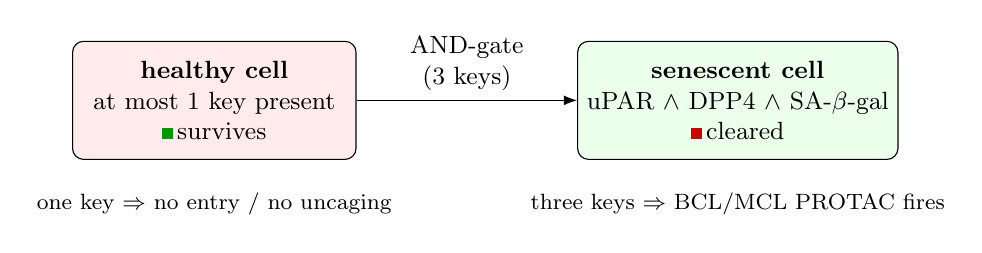
\begin{tikzpicture}[font=\small,node distance=6mm]
\node[draw,rounded corners,fill=red!8,minimum width=3.6cm,minimum height=1.5cm,align=center] (h)
  {\textbf{healthy cell}\\ at most 1 key present\\ \tierGreen{}\,survives};
\node[draw,rounded corners,fill=green!8,minimum width=3.6cm,minimum height=1.5cm,align=center,right=28mm of h] (s)
  {\textbf{senescent cell}\\ uPAR $\wedge$ DPP4 $\wedge$ SA-$\beta$-gal\\ \tierRed{}\,cleared};
\draw[-{Latex}] (h.east) -- node[above,align=center]{AND-gate\\(3 keys)} (s.west);
\node[below=3mm of h,align=center,font=\footnotesize] {one key $\Rightarrow$ no entry / no uncaging};
\node[below=3mm of s,align=center,font=\footnotesize] {three keys $\Rightarrow$ BCL/MCL PROTAC fires};
\end{tikzpicture}
\caption{The SENOLYX-AG AND-gate. Selectivity is multiplicative across three
orthogonal recognition axes; the warhead is a pan-senescent dependency
(BCL-x$_{\mathrm L}$/MCL-1), not an affinity-maximized binder.}
\label{fig:andgate}
\end{figure}

\paragraph{Components (all published chemistry; novelty is composition).}
Warhead: a BCL-x$_{\mathrm L}\to$CRBN PROTAC \citep{pz15227} optionally stacked
with a galacto-caged MCL-1 inhibitor \citep{kotschy2016} --- a pan-senescent
\emph{dependency}, not an affinity target. Cage (axis 1): a $\beta(1,4)$-galactose
cap cleaved by lysosomal SA-$\beta$-gal/GLB1 \citep{navgal2020}. Vehicle
(axes 2--3): a uPAR/DPP4-antibody nanoparticle requiring surface recognition for
entry \citep{amor2020,dpp4}. Event-driven catalytic degradation decouples dose
from toxicity, and CRBN's low platelet expression adds built-in sparing.

\paragraph{First target: the periodontal niche.}
Of the candidate regenerative niches, periodont/gingival tissue uniquely
satisfies all design preconditions: a single dominant CD81$^+$ senescent
fibroblast subtype \citep{perio2024}, a confined local-delivery reservoir (the
periodontal pocket), and a real orthogonal recognition pair. The retina has the
highest predicted $\eta_{\mathrm{neo}}$ but is vascular/epithelial, off the
fibroblast thesis; osteoarthritis is avoided first (UBX0101 precedent).

\paragraph{The finding (Table~\ref{tab:findings}).}
Two axes are ruled out (affinity, clearance-\%), one ceiling is proven
(single-target heterogeneity), one escape is quantified and shown to require
three axes, and a concrete design emerges with realistic
$\sim$13.5--26$\times$ selectivity gated on a single measurable unknown.

\begin{table}[h]
\centering
\caption{Summary of findings against the pre-registered hypotheses.}
\label{tab:findings}
\small
\begin{tabular}{@{}llp{7.4cm}@{}}
\toprule
& Hypothesis & Verdict \\
\midrule
H1 & affinity-orthogonality & \tierBlue{} supported (closed-form + navitoclax) --- affinity axis ruled out \\
H2 & heterogeneity ceiling & \tierBlue{} supported (theorem; no universal dependency) \\
H3 & multiplicative escape & \tierGreen{} supported; \emph{three} axes required for robustness (\texttt{S1}) \\
H4 & gate-variable correction & \tierRed{}$\to$\tierGreen{} clearance-\% ruled out; $\eta_{\mathrm{neo}}$ adopted \\
\bottomrule
\end{tabular}
\end{table}

% =========================================================================
\section{Limitations (honest boundary)}
\label{sec:limits}

All quantitative results are in-silico or literature-grounded. The recognition
ratios, the correlation $\rho$, and the kill-axis $\fs/\fq$ are estimates with
explicit bands, not measurements; the $\eta_{\mathrm{neo}}$ magnitudes and the
parameters $c_{\mathrm{causal}}$, $\tau_{\mathrm{reacc}}$, $\mathrm{AUC_{local}}$
are wet-lab-only. The Hill co-opening haircut is an assumption. The selectivity
\emph{law} (H1) and the ceiling \emph{theorem} (H2) are robust; the design
verdict (H3/H4) is a falsifiable prediction whose single make-or-break is the
three-color flow $\rho$ measurement (\S\ref{sec:rho}). No claim of clinical
efficacy is made; wet-lab is downstream confirmation.

% =========================================================================
\section{Conclusion}
\label{sec:conclusion}

Senolytic selectivity is a differential-dependency quantity, orthogonal to
binding affinity; single-target agents are ceiling-bound by senescence
heterogeneity; the only escape multiplies selectivity across orthogonal
recognition axes, and a direct evaluation shows three axes are required for
robustness. Correcting the downstream gate from clearance-\% to a functional
$\eta_{\mathrm{neo}}$ model reconciles the clinical record. The resulting design,
SENOLYX-AG, is buildable from published chemistry and predicted to reach
$\sim$13.5--26$\times$ selectivity, gated on one measurable correlation. The
campaign wall (ABFE) was not a failure to converge but a signal that the field
had been optimizing the wrong axis.

\paragraph{Acknowledgments.}
Drafted with an autonomous multi-lens research fleet; all verdicts are
literature-grounded and falsifier-fenced.

\bibliographystyle{unsrtnat}
\bibliography{references}

\end{document}
